\subsection{Company History}

Founded in 2021 at Egypt-Japan University of Science and Technology (E-JUST), the club began with courses and workshops to support robotics learners. Over time, members engaged in large-scale projects, forming specialized teams for competitions.

\hspace{10pt} A major milestone was the \textbf{formation of the first ROV team in 2023}, which competed in MATE ROV 2023 and won the \textbf{"No Pain, No Gain"} award. The team improved further in MATE ROV 2024, excelling in underwater tasks.

\begin{figure}[h]
    \centering
    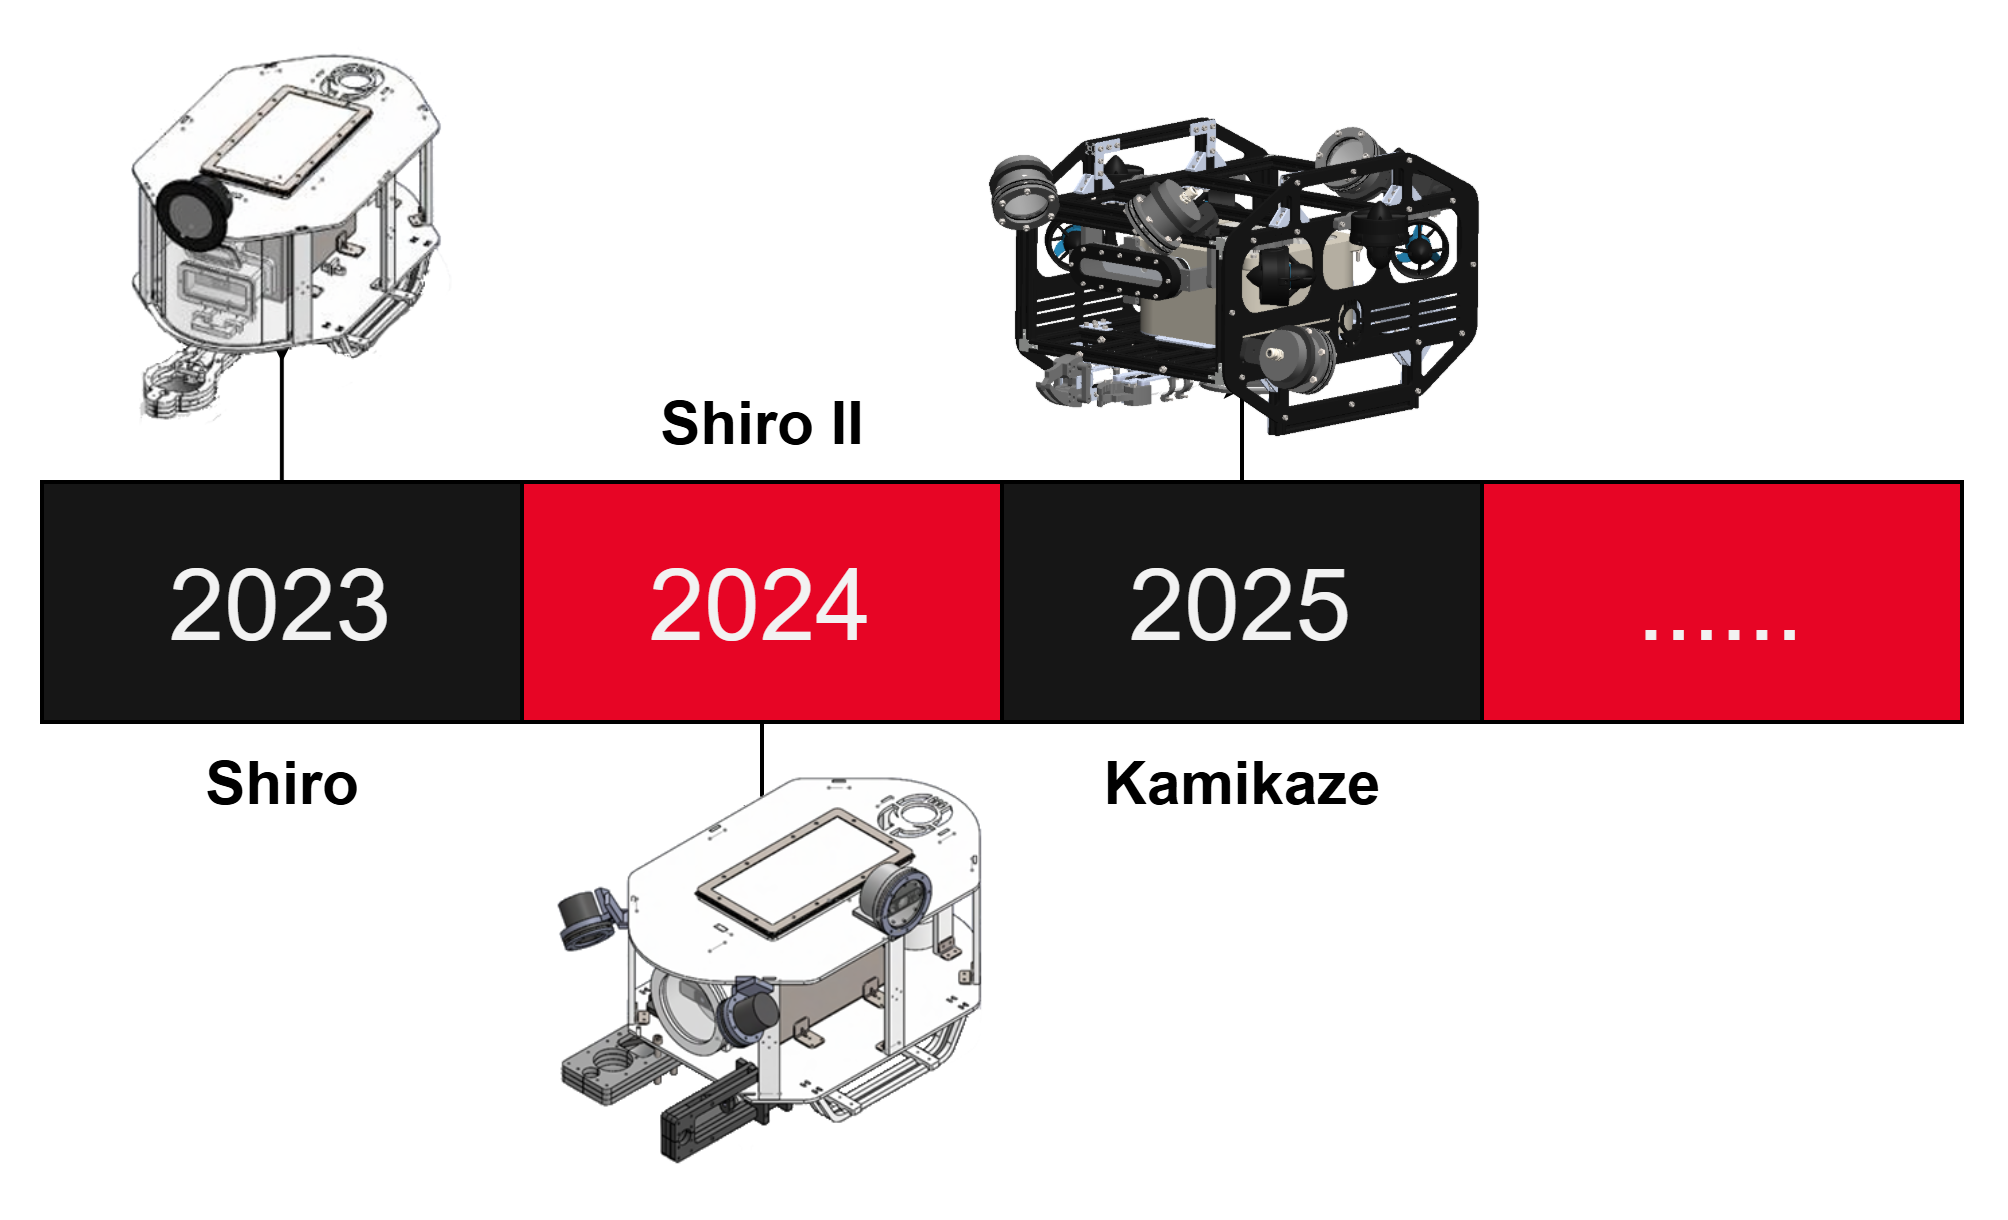
\includegraphics[width=\columnwidth]{Sections/5Logistics/images/ROVs over the years (1).png}
    \caption{EJUST Robotics Club ROVs over years.}
    \label{fig:over_years}
\end{figure}

\hspace{10pt} The club unites students from various fields, following a structured training process to ensure knowledge transfer and skill development:
\vspace{-0.5\baselineskip}
\begin{enumerate}[leftmargin=0pt, itemindent=20pt]
    \setlength{\itemsep}{0pt}
    \item \textbf{General Training:} New members learn robotics fundamentals, including design, electronics, programming, and control.
    \item \textbf{Evaluation:} Members are assessed to identify strengths and roles.
    \item \textbf{Team Selection:} Based on performance, members join the ROV or other teams.
\end{enumerate}

The E-JUST ROV team has \textbf{47 members} divided into:
\vspace{-0.5\baselineskip}
\begin{itemize}[leftmargin=0pt, itemindent=20pt]
    \setlength{\itemsep}{0pt}
    \item \textbf{Technical Sector:} Focuses on ROV design and development.
    \item \textbf{Non-Technical Sector:} Manages operations and outreach.
\end{itemize}
This year, the team developed \textbf{Kamikaze}, our custom ROV, using Agile methodology and cloud-based collaboration.